%\documentclass[a4paper, 10pt]{article}
\documentclass[a4paper, 11pt,twocolumn]{article}


\usepackage{lipsum,lineno}
\usepackage{graphicx}
\usepackage{subcaption}
\title{Latex Document Types}
\author{Debadatta Mishra}
\date{}
\begin{document}
\maketitle
\begin{abstract}
\lipsum[15]
\end{abstract}    
\section{Introduction}
\lipsum[70]


\section{Motivation}

\begin{figure}
\centering
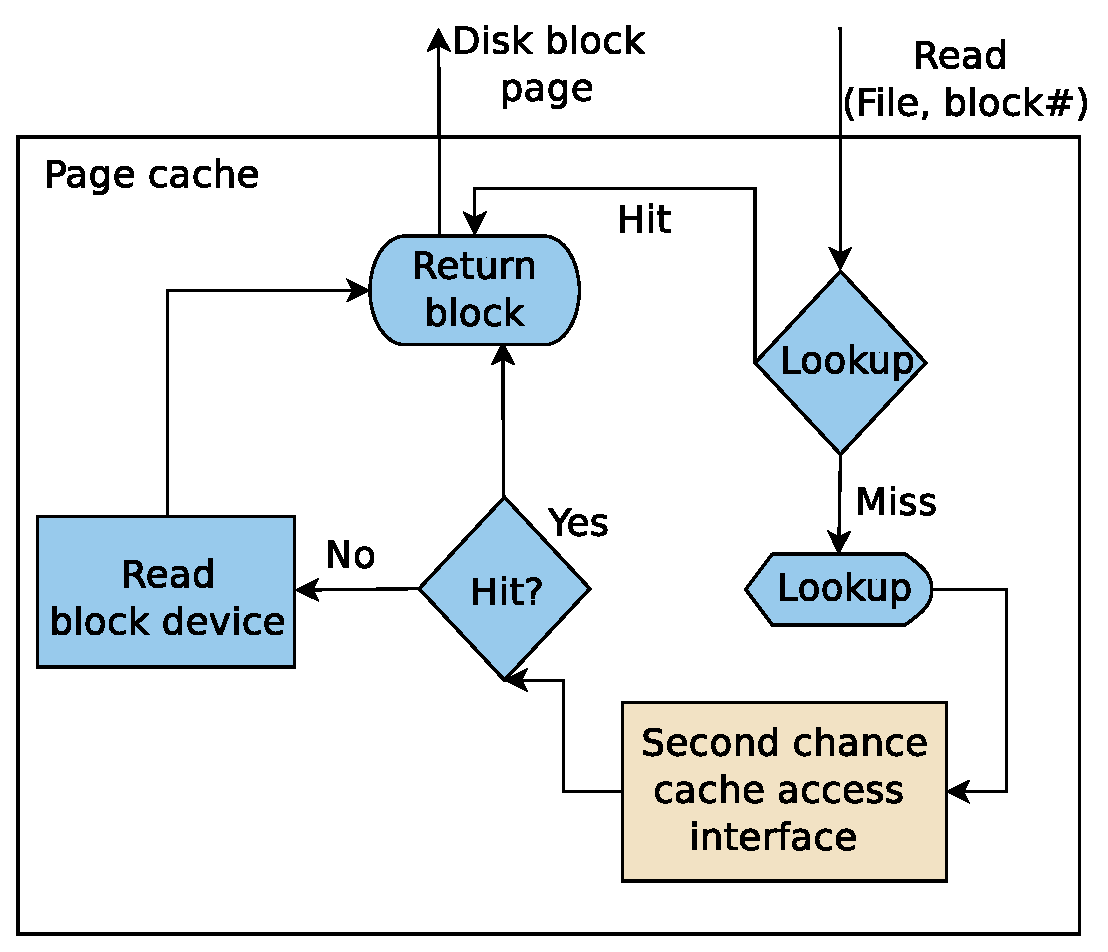
\includegraphics[width=0.35\textwidth]{cc_get.eps}
 \caption{This is a single figure.}
 \label{fig:cc_get}
\end{figure}

As shown in Figure~\ref{fig:cc_get}, we conclude nothing!
\lipsum[50]
\subsection{Why learn latex?}
\lipsum[50]

\lipsum[50]


\lipsum[50]

\subsubsection{Now you know why latex, Really?}
\lipsum[50]

\lipsum[50]

\section{Design}
\begin{figure*}
\centering
\begin{subfigure}{0.41\linewidth}
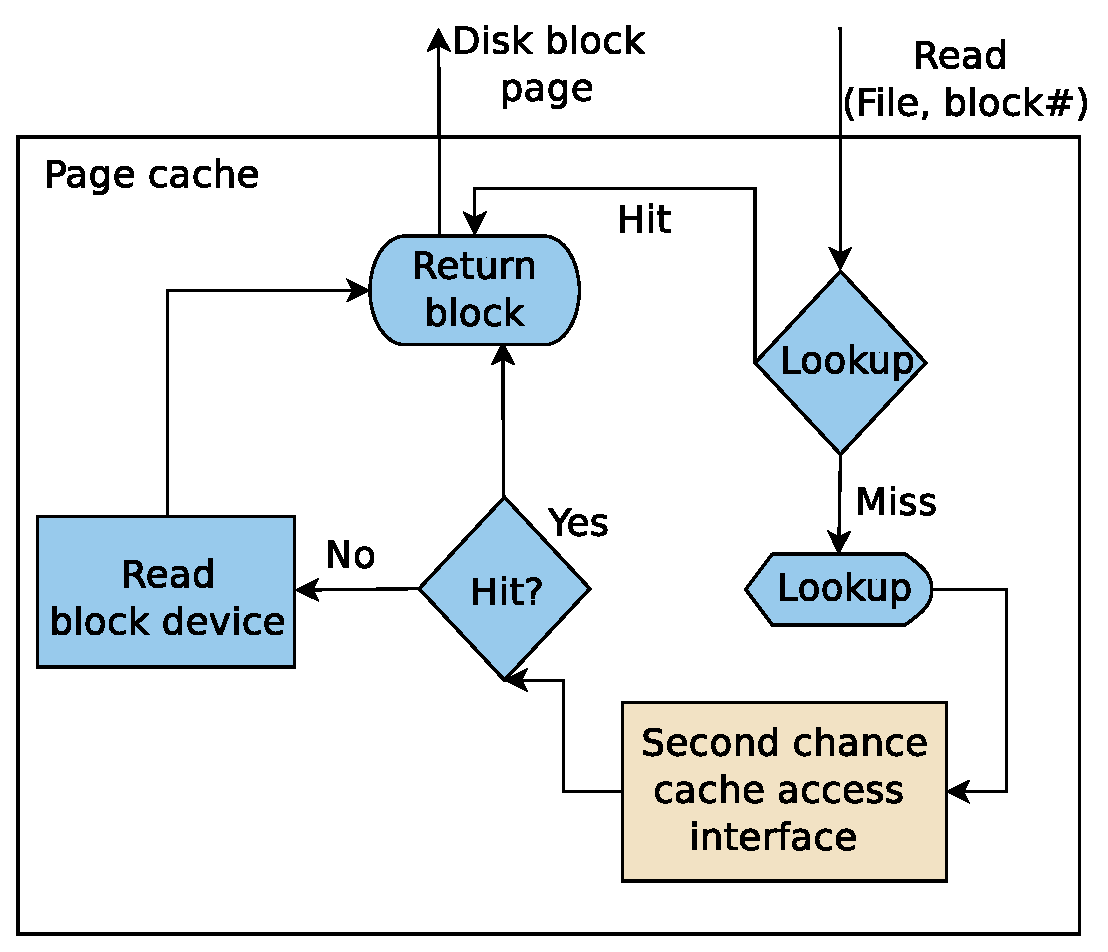
\includegraphics[width=\columnwidth]{cc_get.eps}
 \caption{I am part-1}
 \label{fig:part1}
\end{subfigure} \hfill
%
\begin{subfigure}{0.41\linewidth}
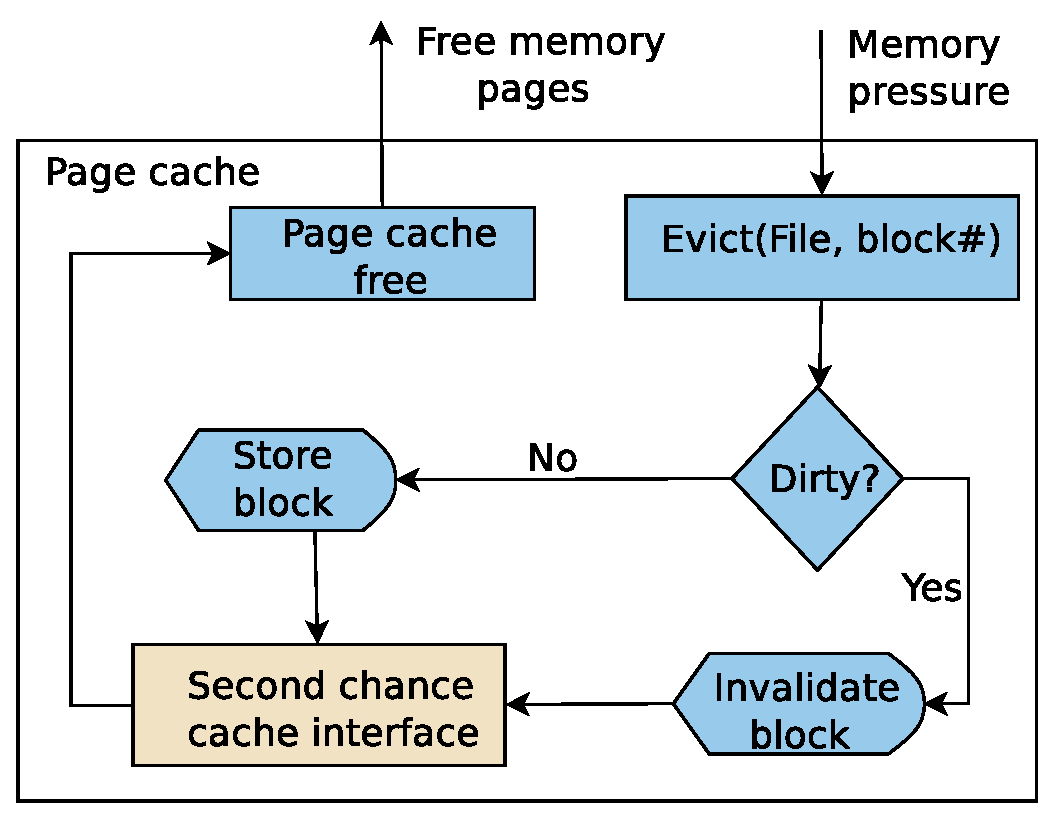
\includegraphics[width=\columnwidth]{evict.eps}
 \caption{I am part-2}
 \label{fig:part2}
\end{subfigure} \hfill
%
\caption{This is a composite figure containing two sub-figures.}
\label{fig:composite}
\end{figure*}

As shown in Figure~\ref{fig:composite}, there are two subcomponents---Part(1) in Figure~\ref{fig:part1}
and Part(2) in Figure~\ref{fig:part2}.
\lipsum[50]

\lipsum[50]

\begin{table}[t]
\scriptsize
\begin{center}
\begin{tabular}{|c|c|c|c|}
\hline
{\bf Assign-} & {\bf Topic} & {\bf \#of} & {\bf Avg.} \\
{\bf -ment} & & {\bf submissions} & {\bf marks (/30)} \\
\hline
\hline
I & Bash & 90 & 20 \\
%\hline
II & AWK &  80 & 18.5 \\
%\hline
III & Python & 100 & 24 \\
%\hline
IV & Latex & 110 & 29 \\
\hline
\end{tabular}
\caption{This is a simple table showing assignment submission statistics.}
\label{table:simple}
\end{center}
\end{table}

Table~\ref{table:simple} shows phony data regarding CS251 assignment submission.
\lipsum[50]

\section{Evaluation}
\begin{table*}[t]
\scriptsize
\begin{center}
\begin{tabular}{|c|c|c|c|c|c|c|c|c|c|}
\cline{2-10}
\multicolumn{1}{c}{} & \multicolumn{3}{|c|}{\bf 2015} & \multicolumn{3}{c|}{\bf 2016} & \multicolumn{3} {c|}{\bf 2017}\\
\cline{1-10}
\multicolumn{1}{|c|}{} & {\bf \#of } & {\bf Semester} & {\bf Avg.} & {\bf \#of } & {\bf Semester} & {\bf Avg.} & {\bf \#of } & {\bf Semester} & {\bf Avg.}\\
%
\multicolumn{1}{|c|}{\bf Course} & {\bf Students} & {} & {\bf Marks} & {\bf Students} & {} & {\bf Marks}& {\bf Students} & {} & {\bf Marks} \\
%
\hline
\hline
CS101 & 500 & Both & 80 & 480 & Both & 81 & 520 & Both & 88\\
\hline
CS251 & 122 &  Even & 80 & 111 & Even & 81 &Even & 109 & 70 \\
\hline
CS220 & 122 &  Both & 84 & 111 & Even & 81 & Odd & 119 & 70 \\
\hline
CS330 & 100 &  Odd & 87 & 115 & Odd & 90 & Odd & 150 & 70 \\
\hline
CS698 & 15 & Odd & 65 & --- & --- & --- & 23 & Even & 76 \\
\hline
\end{tabular}
\caption{Student registration details over the last 3 years for different courses
offered by Computer Science Department.}
\label{table:big}
\end{center}
\end{table*}
\lipsum[50]


Table~\ref{table:big}, a page wide table shows the registration details of the 
students.

\lipsum
\section{Conclusion}
\lipsum[30]

\end{document}
